\chapter{पौधों का कायिक विकास: विभज्योतक और वृद्धि}\label{ch:b2:plant-meristems}

जो बलूत उस गिरजाघर के बनते समय अंकुर भर था वह आज भी हर वर्ष \omterm{def:b2:plant-meristems:wood}{काष्ठ} का एक
वलय जोड़ रहा है, आज भी हर वसंत नई पत्तियाँ खोल रहा है, आज भी मिट्टी में
नए मूल-शीर्ष धकेल रहा है। कोई प्राणी यह नहीं करता; कोई घोड़ा चार वर्ष
पर बढ़ना बंद कर देता है। भेद यह है कि पौधा हर प्ररोह और हर जड़ के सिरे
पर, और हर तने के भीतर एक पतले बेलन में, भ्रूणीय कोशिकाओं की छोटी आबादियाँ
रखता है --- यानी \emph{\omterm{def:b2:plant-meristems:meristem}{विभज्योतक}} --- जो कभी विभाजित होना बंद नहीं
करतीं और जो उस पौधे का शरीर जब तक वह जीए तब तक बाहर और ऊपर की ओर गढ़ती
रहती हैं। यह अध्याय देखता है कि दोनों शीर्षस्थ \omterm{def:b2:plant-meristems:meristem}{विभज्योतक} कैसे संगठित और
नियंत्रित हैं, कोई पादप कोशिका कैसे बढ़ती है, हॉर्मोन किसी प्ररोह का आकार
कैसे तय करते हैं, और कोई तना कैसे मोटा होता है।

\section{विभज्योतक}

\begin{definition}[विभज्योतक और वृद्धि के दो प्रकार]\label{def:b2:plant-meristems:meristem}
\index{विभज्योतक}\index{प्ररोह शीर्षस्थ विभज्योतक}\index{मूल शीर्षस्थ विभज्योतक}\index{कैंबियम}
\emph{विभज्योतक} छोटी, अविभेदित, विभाजित होती कोशिकाओं की ऐसी आबादी है
जो उस पौधे के पूरे जीवन भर बनी रहती है और जिससे उसके सारे ऊतक निकलते
हैं। हर प्ररोह के सिरे पर \emph{प्ररोह शीर्षस्थ विभज्योतक} (SAM)
पत्तियाँ, तना और, ऋतु आने पर, \omterm{def:b2:angiosperm-reproduction:flower}{पुष्प} बनाता है;
हर मूल-शीर्ष के पीछे \emph{मूल शीर्षस्थ विभज्योतक} (RAM) उस
जड़ को बनाता है; और मिलकर वे \emph{प्राथमिक वृद्धि} चलाते हैं, यानी उस
पौधे का लंबा होना। \emph{पार्श्व विभज्योतक} --- यानी \emph{\omterm{def:b2:plant-meristems:wood}{संवहनी
कैंबियम}} और \emph{कॉर्क कैंबियम}, जो तनों तथा जड़ों के भीतर पतले बेलन
हैं --- \emph{द्वितीयक वृद्धि} चलाते हैं, यानी वह मोटापन जो
\omterm{def:b2:plant-meristems:wood}{काष्ठ} और \omterm{def:b2:plant-meristems:wood}{छाल} बनाता है। इसलिए पादप वृद्धि \emph{अनिश्चित} है:
वे विभज्योतक अनिश्चित काल तक चल सकते हैं, और वह पौधा एक खंडीय
जीव है, जो पत्ती--पर्वसंधि--पर्वसंधि-अंतराल--कलिका की इकाई तब तक दोहराता
है जब तक परिस्थितियाँ अनुमति दें। हर कक्षस्थ कलिका एक प्रसुप्त SAM है,
इसलिए कोई पौधा हज़ारों आरक्षित वृद्धि-बिंदु ढोता है।
\end{definition}

\begin{proposition}[प्ररोह शीर्ष]\label{prop:b2:plant-meristems:sam}
\index{पर्णविन्यास}\index{पर्ण प्राथमिकांग}\index{प्लास्टोक्रॉन}
SAM मिलिमीटर के दसवें भाग जितना चौड़ा एक गुंबद है, जो कुछ सौ
कोशिकाओं का है। उसकी बाहरी एक या दो परतें (\emph{ट्यूनिका}) केवल
सतह के तल में विभाजित होती हैं और अधिचर्म देती हैं; और नीचे का पिंड
(\emph{कॉर्पस}) हर तल में विभाजित होता है। चोटी पर धीरे विभाजित होती
\omterm{def:b2:cell-differentiation:differentiation}{स्तंभ कोशिकाओं} का \emph{केंद्रीय क्षेत्र} तेज़ विभाजित होती कोशिकाओं के
एक \emph{परिधीय क्षेत्र} को पालता है, जहाँ \emph{\omterm{prop:b2:plant-meristems:sam}{पर्ण
प्राथमिकांग}} नियमित काल-अंतरालों पर (यानी
\emph{प्लास्टोक्रॉन} पर, जो घंटों से दिनों का है) और उस गुंबद के चारों
ओर नियमित कोणों पर (यानी \emph{पर्णविन्यास}: सम्मुख, चक्रित, या
\qty{137.5}{\degree} के स्वर्णिम कोण पर सर्पिल, जो हर नई पत्ती को बाक़ी
पत्तियों द्वारा छोड़ी सबसे बड़ी ख़ाली जगह में बिठा देता है) उभारों के रूप
में उठते हैं। नीचे कोई \emph{पर्शुका क्षेत्र} मज्जा बनाता है
और तने को लंबा करता है। कोई प्राथमिकांग वहीं बनता है जहाँ हॉर्मोन ऑक्सिन
सतही परत में जमा हो, और बढ़ते-बढ़ते वह अपने परिवेश से ऑक्सिन खींच लेता
है, और इसीलिए अगला प्राथमिकांग उससे यथासंभव दूर उठता है: वह प्रतिरूप
स्वयं-संगठित है।
\end{proposition}

\begin{omfigure}
\begin{tikzpicture}[every node/.style={font=\scriptsize}]
  % dome
  \draw[thick, fill=omExo!12] (-2.2,0) .. controls (-2.2,1.6) and (-0.8,2.6) .. (0,2.6) .. controls (0.8,2.6) and (2.2,1.6) .. (2.2,0) -- (2.2,-1.4) -- (-2.2,-1.4) -- cycle;
  % tunica layers
  \draw[thick, omDef] (-2.2,0) .. controls (-2.2,1.5) and (-0.8,2.45) .. (0,2.45) .. controls (0.8,2.45) and (2.2,1.5) .. (2.2,0);
  \draw[thick, omDef] (-2.05,0) .. controls (-2.05,1.35) and (-0.75,2.3) .. (0,2.3) .. controls (0.75,2.3) and (2.05,1.35) .. (2.05,0);
  % zones
  \draw[thick, dashed, omThm, fill=omThm!15] (0,1.75) ellipse (0.6 and 0.55);
  \draw[thick, dashed, omProp] (0,0.9) ellipse (1.6 and 1.35);
  \draw[thick, dashed, omExo!70!black] (-0.9,-0.9) rectangle (0.9,-0.1);
  % primordia
  \draw[thick, fill=omExo!40] (-2.2,0.4) .. controls (-2.5,1.4) and (-1.6,1.9) .. (-1.55,1.3) .. controls (-1.5,0.9) and (-1.9,0.6) .. (-2.2,0.4);
  \draw[thick, fill=omExo!40] (2.2,0.2) .. controls (2.7,1.0) and (2.1,1.5) .. (1.75,1.1) .. controls (1.6,0.8) and (1.9,0.5) .. (2.2,0.2);
  % labels
  \draw (0.4,2.1) -- (3.2,2.6) node[right, align=left] {केंद्रीय क्षेत्र:\\धीरे विभाजित होती स्तंभ कोशिकाएँ};
  \draw (1.3,0.5) -- (3.2,1.4) node[right, align=left] {परिधीय क्षेत्र:\\तेज़ विभाजन, पर्ण प्राथमिकांग};
  \draw (0.6,-0.5) -- (3.2,0.0) node[right, align=left] {पर्शुका क्षेत्र: मज्जा,\\तने का दीर्घीकरण};
  \draw (-1.7,1.5) -- (-3.0,2.4) node[left, align=right] {पर्ण\\प्राथमिकांग};
  \draw (-1.2,2.05) -- (-3.0,1.2) node[left, align=right] {ट्यूनिका: केवल\\सतही विभाजन};
  \draw (2.2,0.7) -- (3.2,-1.0) node[right, align=left] {अगला प्राथमिकांग,\\\qty{137.5}{\degree} घूमकर};
\end{tikzpicture}

{\small काट में \omterm{def:b2:plant-meristems:meristem}{प्ररोह शीर्षस्थ विभज्योतक}: किसी कॉर्पस के ऊपर एक या दो
सतही परतों की ट्यूनिका, चोटी पर \omterm{def:b2:cell-differentiation:differentiation}{स्तंभ कोशिकाओं} का एक केंद्रीय क्षेत्र,
एक परिधीय क्षेत्र जहाँ \omterm{prop:b2:plant-meristems:sam}{पर्ण प्राथमिकांग} उभरते हैं, और नीचे एक पर्शुका
क्षेत्र।}
\end{omfigure}

\begin{omfigure}
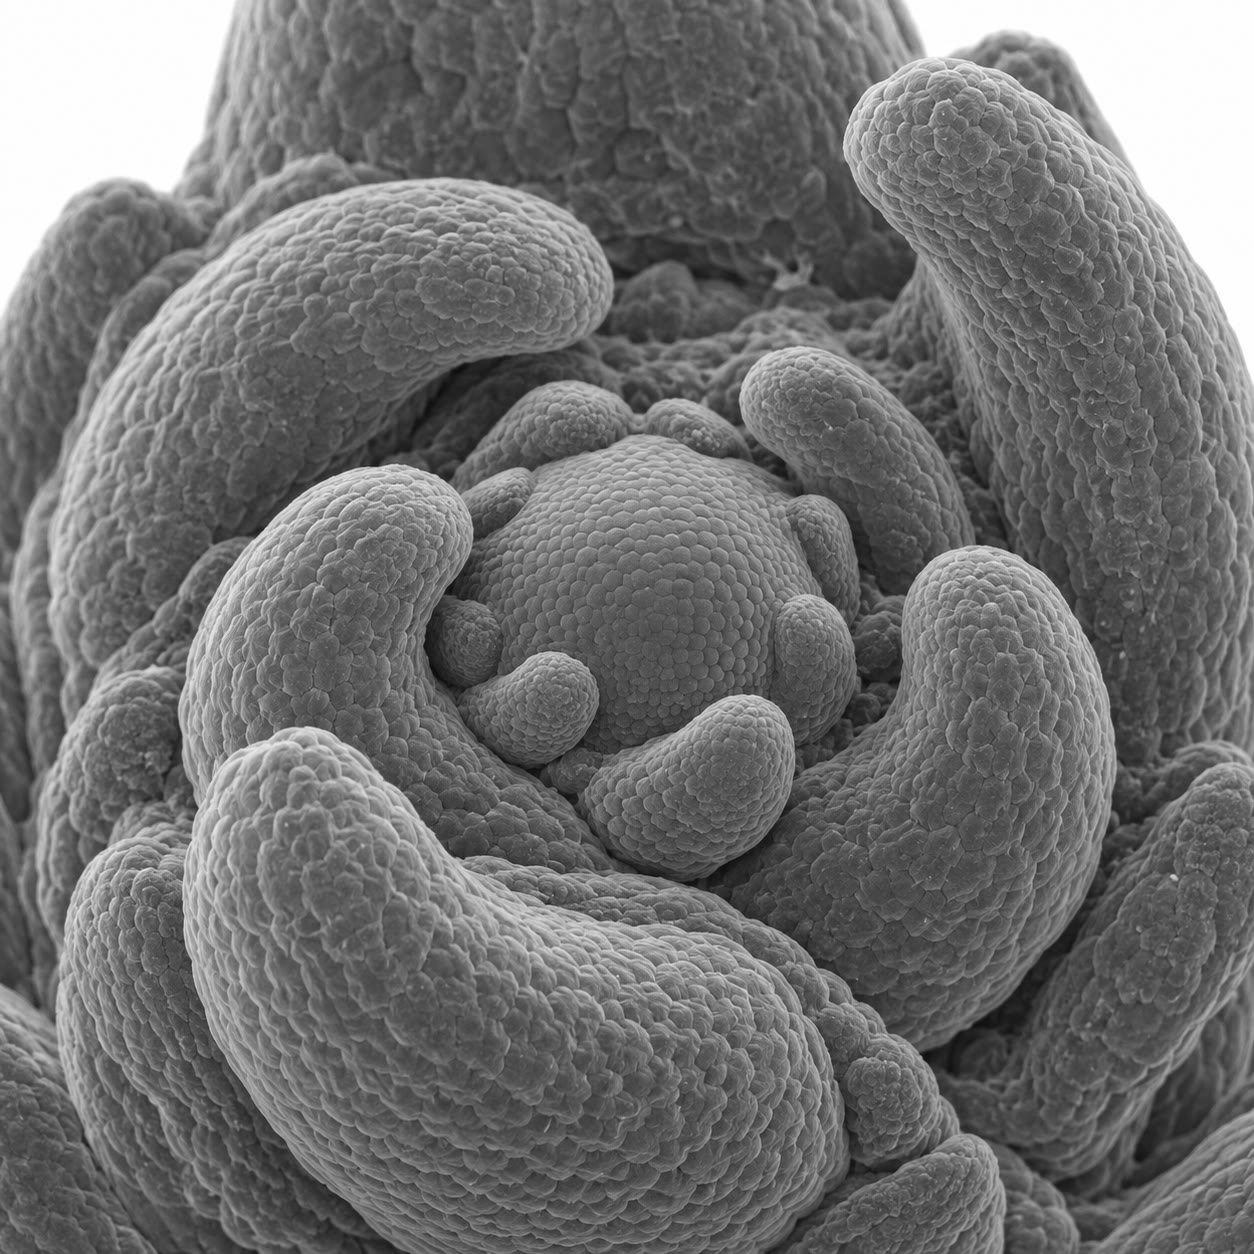
\includegraphics[width=0.44\linewidth]{images/book4/ai/b4-13-shoot-apex-sem.jpg}

{\small क्रमवीक्षी इलेक्ट्रॉन सूक्ष्मदर्शी के नीचे एक प्ररोह शीर्ष:
\omterm{def:b2:plant-meristems:meristem}{विभज्योतक} का चिकना गुंबद और उसके चारों ओर \omterm{prop:b2:plant-meristems:sam}{पर्ण प्राथमिकांगों} का सर्पिल,
जिसमें हर नया सबसे चौड़ी ख़ाली जगह में बिठाया गया है।}
\end{omfigure}

\begin{proposition}[स्तंभ कोशिकाएँ बनाए रखना: एक प्रतिपुष्टि चक्र]\label{prop:b2:plant-meristems:wus}
\index{WUSCHEL}\index{CLAVATA}\index{ऋण प्रतिपुष्टि!विभज्योतक}
स्तंभ-कोशिका भंडार का आकार दो जीनों के बीच के एक चक्र से अचर रखा जाता
है। केंद्रीय क्षेत्र के ठीक नीचे की कोशिकाएँ
\omterm{prop:b2:cell-differentiation:transcriptional}{अनुलेखन कारक} \emph{WUSCHEL} (WUS) अभिव्यक्त करती हैं, जिसका उत्पाद ऊपर
की कोशिकाओं में जाकर उन्हें \omterm{def:b2:cell-differentiation:differentiation}{स्तंभ कोशिकाएँ} बनाए रखता है; और वे \omterm{def:b2:cell-differentiation:differentiation}{स्तंभ
कोशिकाएँ} बदले में एक छोटा पेप्टाइड, \emph{CLAVATA3} (CLV3), स्रावित
करती हैं, जो नीचे विसरित होता है, WUS अभिव्यक्त करती कोशिकाओं में किसी
ग्राही काइनेज़ (CLV1) से बँधता है और WUS को दबा देता है। अधिक \omterm{def:b2:cell-differentiation:differentiation}{स्तंभ
कोशिकाओं} का अर्थ है अधिक CLV3, कम WUS, और कम \omterm{def:b2:cell-differentiation:differentiation}{स्तंभ
कोशिकाएँ}; और कम \omterm{def:b2:cell-differentiation:differentiation}{स्तंभ कोशिकाओं} का अर्थ है कम CLV3, अधिक WUS, और अधिक
\omterm{def:b2:cell-differentiation:differentiation}{स्तंभ कोशिकाएँ}। इस तरह वह भंडार एक नियमित राशि है, ठीक
\cref{ch:b2:reproductive-hormones} की गोनैडोट्रोपिनों की तरह, और वही
तर्क --- नियमित आबादी का कोई संकेत उस कारक को दबाता है जो उसे बनाता है
--- मूल \omterm{def:b2:plant-meristems:meristem}{विभज्योतक} को भी थामे रखता है।
\end{proposition}
\begin{proof}[प्रमाण-सामग्री]
Arabidopsis के \emph{clavata} उत्परिवर्तियों (क्लार्क,
मेयरोविट्ज़, 1990 का दशक) के \omterm{def:b2:plant-meristems:meristem}{विभज्योतक} फूलकर सामान्य से कई गुना बड़े हो
जाते हैं, और उनमें अतिरिक्त पत्तियाँ, अतिरिक्त पुष्प-अंग तथा फ़ैसिएटेड
(चपटे, फ़ीते जैसे) तने होते हैं: यानी ब्रेक जाता रहा। \emph{wuschel}
उत्परिवर्ती ऐसा \omterm{def:b2:plant-meristems:meristem}{विभज्योतक} बनाते हैं जो कुछ पत्तियों के बाद रुक जाता है
और फिर नए बनाता है, और हर एक बारी-बारी रुक जाता है: यानी त्वरक जाता
रहा। दोहरे उत्परिवर्ती में \emph{wuschel} का \omterm{def:b2:meiosis-heredity:vocabulary}{लक्षण-प्ररूप} जीतता है, जो
WUS को CLV के नीचे रखता है; और किसी वन्य-प्ररूप शीर्ष पर लगाया गया CLV3
पेप्टाइड घंटों में WUS दबा देता है।
\end{proof}

\begin{proposition}[मूल शीर्ष]\label{prop:b2:plant-meristems:ram}
\index{मूल टोप}\index{निष्क्रिय केंद्र}\index{दीर्घीकरण क्षेत्र}\index{मूलरोम}
कोई जड़ ऐसे \omterm{def:b2:plant-meristems:meristem}{विभज्योतक} से बढ़ती है जो किसी \emph{\omterm{prop:b2:plant-meristems:ram}{मूल टोप}} के पीछे
सुरक्षित है, और जिसकी कोशिकाएँ मिट्टी में सिरे के धँसने के साथ झड़ती
जाती हैं तथा जो चिकनाई देता श्लेष्म स्रावित करता है और गुरुत्व भाँपता है
(उसकी कोशिकाओं में बैठते मंड-कण)। उस \omterm{def:b2:plant-meristems:meristem}{विभज्योतक} के केंद्र में
कुछ सौ कोशिकाओं का एक \emph{\omterm{prop:b2:plant-meristems:ram}{निष्क्रिय केंद्र}} कभी-कभार ही विभाजित होता
है; वह अपने चारों ओर की आद्य कोशिकाओं को --- टोप की, अधिचर्म की,
वल्कुट की और संवहनी बेलन की --- \omterm{def:b2:cell-differentiation:differentiation}{स्तंभ कोशिकाएँ} बनाए रखता है, ठीक जैसे
WUS प्ररोह की कोशिकाओं को। \omterm{def:b2:plant-meristems:meristem}{विभज्योतक} के पीछे \emph{\omterm{prop:b2:plant-meristems:ram}{दीर्घीकरण
क्षेत्र}} आता है, यानी कुछ मिलिमीटर जिनमें कोशिकाएँ दस से
बीस गुना लंबी होती हैं और सिरे को आगे धकेलती हैं; फिर \emph{\omterm{def:b2:cell-differentiation:differentiation}{विभेदन}
क्षेत्र}, जहाँ अधिचर्म \emph{मूलरोम} उगाता है और जाइलम तथा
फ्लोएम परिपक्व होते हैं। पार्श्व जड़ें सिरे पर नहीं बल्कि
परिरंभ से उठती हैं, यानी परिपक्व जड़ के भीतर गहरे, जाइलम ध्रुवों के
सामने, और वल्कुट से होकर बाहर धकेलती हैं। प्ररोह में बना और नीचे ढोया
गया ऑक्सिन उस सिरे पर जमा होता है और पूरी व्यवस्था संगठित करता है; और
वह \omterm{prop:b2:plant-meristems:ram}{निष्क्रिय केंद्र} उसके अधिकतम पर बैठता है।
\end{proposition}

\begin{omfigure}
\begin{tikzpicture}[every node/.style={font=\scriptsize}]
  % root outline
  \draw[thick, fill=omExo!10] (-1.0,4.5) -- (-1.0,0.6) .. controls (-1.0,-0.4) and (1.0,-0.4) .. (1.0,0.6) -- (1.0,4.5);
  % root cap
  \draw[thick, fill=omExo!45] (-0.9,0.8) .. controls (-1.1,-0.1) and (1.1,-0.1) .. (0.9,0.8) .. controls (0.5,0.4) and (-0.5,0.4) .. (-0.9,0.8);
  % meristem
  \fill[omThm!25] (-0.85,0.8) rectangle (0.85,1.7);
  \fill[omThm!70] (0,0.95) ellipse (0.25 and 0.12);
  % elongation zone
  \fill[omProp!20] (-0.85,1.7) rectangle (0.85,3.0);
  % differentiation zone with root hairs and vascular strand
  \fill[omDef!15] (-0.85,3.0) rectangle (0.85,4.5);
  \fill[omDef!50] (-0.15,3.0) rectangle (0.15,4.5);
  \foreach \y in {3.2,3.5,3.8,4.1,4.4} { \draw[omDef!80!black] (1.0,\y) -- (1.7,\y+0.1); \draw[omDef!80!black] (-1.0,\y) -- (-1.7,\y+0.1); }
  % lateral root primordium
  \draw[thick, fill=omThm!30] (0.15,4.0) .. controls (0.5,3.9) and (0.8,4.1) .. (0.9,4.3) .. controls (0.7,4.35) and (0.4,4.3) .. (0.15,4.3);
  % labels
  \draw (0.5,0.4) -- (2.2,0.2) node[right] {मूल टोप};
  \draw (0.25,0.95) -- (2.2,0.9) node[right] {निष्क्रिय केंद्र};
  \draw (0.85,1.4) -- (2.2,1.5) node[right] {विभज्योतक (विभाजन)};
  \draw (0.85,2.4) -- (2.2,2.3) node[right, align=left] {दीर्घीकरण क्षेत्र:\\कोशिकाएँ $10\times$ लंबी होती हैं};
  \draw (1.5,3.6) -- (2.2,3.4) node[right] {मूलरोम};
  \draw (0.0,4.2) -- (2.2,4.2) node[right] {संवहनी बेलन};
  \draw (0.7,4.3) -- (2.2,4.9) node[right, align=left] {पार्श्व मूल प्राथमिकांग\\(परिरंभ से)};
  \draw[->, thick] (-2.4,4.5) -- (-2.4,0.6); \node[left, rotate=90, anchor=south] at (-2.5,2.5) {ऑक्सिन सिरे की ओर बहती है};
\end{tikzpicture}

{\small मूल-शीर्ष: टोप, अपने \omterm{prop:b2:plant-meristems:ram}{निष्क्रिय केंद्र} सहित \omterm{def:b2:plant-meristems:meristem}{विभज्योतक},
\omterm{prop:b2:plant-meristems:ram}{दीर्घीकरण क्षेत्र}, और मूलरोमों तथा परिपक्व वाहिकाओं सहित \omterm{def:b2:cell-differentiation:differentiation}{विभेदन} क्षेत्र।
पार्श्व जड़ें भीतर गहरे, परिरंभ से आरंभ होती हैं।}
\end{omfigure}

\begin{omfigure}
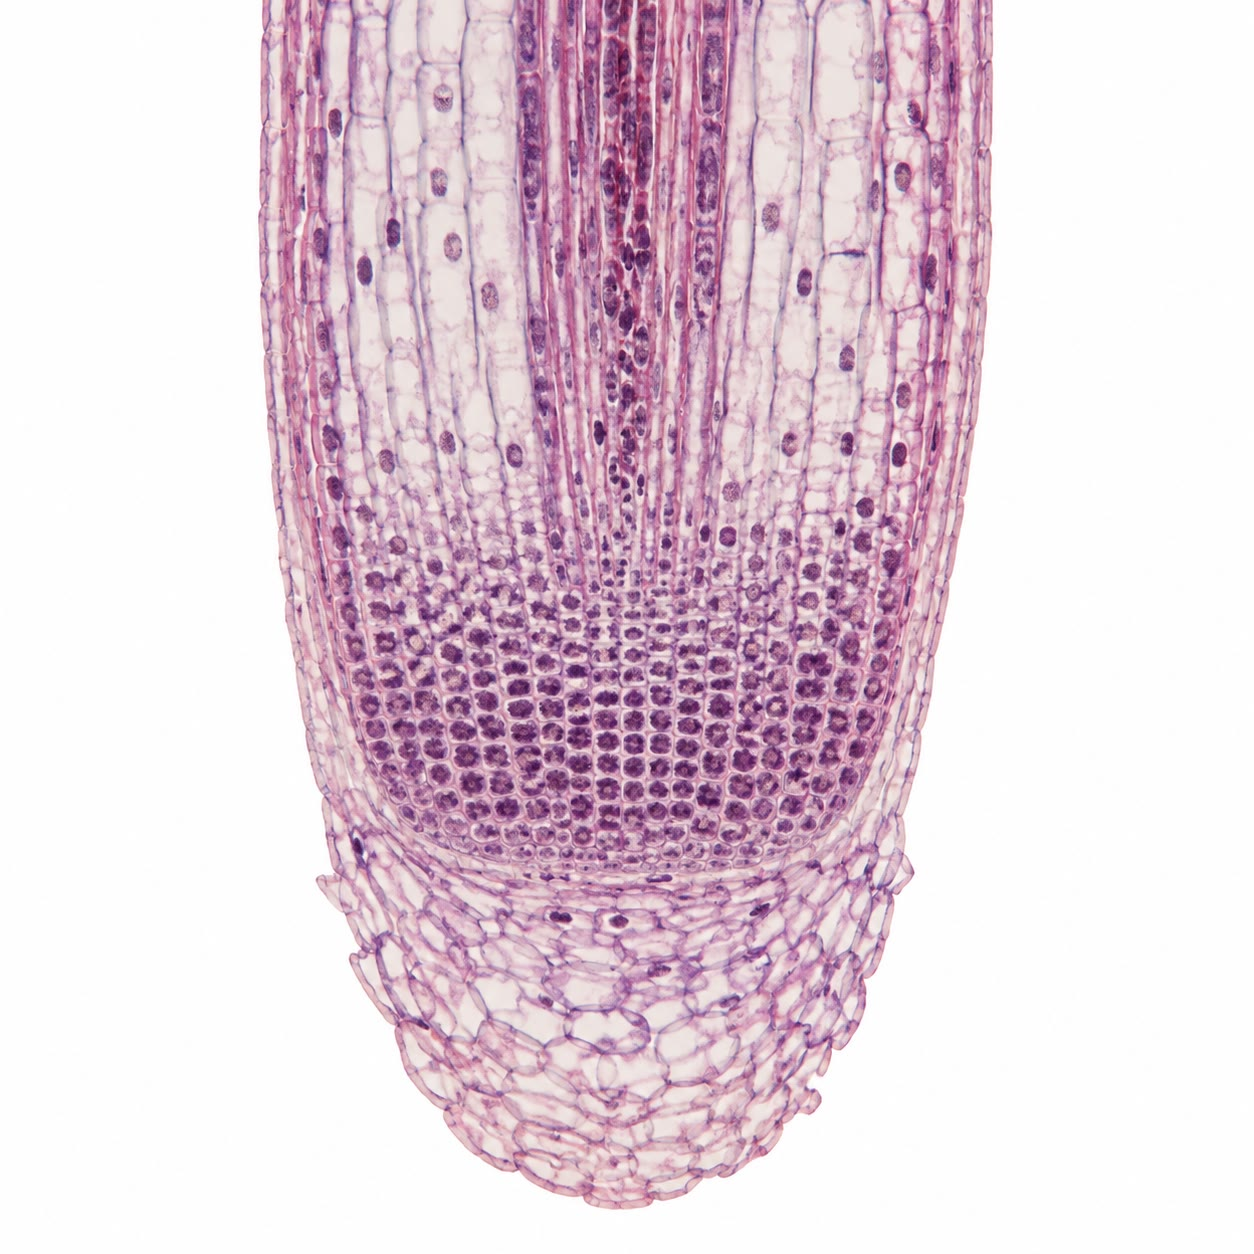
\includegraphics[width=0.42\linewidth]{images/book4/ai/b4-13-root-tip.jpg}

{\small अनुदैर्घ्य काट में एक मूल-शीर्ष: टोप की ढीली कोशिकाएँ,
गहरे केंद्रकों वाला सघन \omterm{def:b2:plant-meristems:meristem}{विभज्योतक}, और ऊपर लंबी होती
कोशिकाएँ।}
\end{omfigure}

\section{कोई पादप कोशिका कैसे बढ़ती है}

\begin{theorem}[लॉकहार्ट समीकरण]\label{thm:b2:plant-meristems:lockhart}
\index{स्फीति}\index{कोशिका भित्ति!विस्तार्यता}\index{लॉकहार्ट समीकरण}
कोई पादप कोशिका अपनी ही अंतर्वस्तु के दाब में अपनी भित्ति खींचकर बढ़ती
है। वह भित्ति किसी देहली स्फीति $Y$ से ऊपर ही अप्रतिवर्ती रूप से झुकती
है, और तब उस आधिक्य के समानुपाती दर से: $L$ लंबाई की किसी कोशिका की
सापेक्ष वृद्धि दर है
\[
\frac{1}{L}\frac{\mathrm{d}L}{\mathrm{d}t} = \phi\,(P - Y) \quad (P > Y),
\]
जिसमें $P$ स्फीति दाब है और $\phi$ उस भित्ति की
\emph{विस्तार्यता}। इसलिए वृद्धि दो ओर से नियंत्रित है:
जल से, जो $P$ तय करता है (मुरझाती कोशिका बढ़ना बंद कर देती है), और उस
भित्ति से, जो $\phi$ तथा $Y$ तय करती है --- और हॉर्मोन उसी भित्ति पर
काम करते हैं। ऑक्सिन कोशिकाओं से भित्ति में प्रोटॉन पंप कराती है; और वह
अम्ल \emph{एक्सपैंसिन} सक्रिय कर देता है, यानी वे प्रोटीन जो सेलुलोस
तंतुकों और आधात्री के बीच के बंध ढीले करते हैं, और मिनटों में $\phi$
चढ़ा तथा $Y$ गिरा देते हैं (\emph{अम्ल वृद्धि})। $\phi =
\qty{0.1}{h^{-1}.MPa^{-1}}$, $Y = \qty{0.3}{MPa}$ और $P =
\qty{0.6}{MPa}$ के साथ कोई कोशिका घंटे भर में \qty{3}{\%} लंबी होती है
और दिन भर में दुगुनी; और किसी जड़ के \omterm{prop:b2:plant-meristems:ram}{दीर्घीकरण क्षेत्र} में, जहाँ दरें कई
गुना अधिक हैं, कोई कोशिका कुछ ही घंटों में दस गुना लंबी हो जाती है।
\end{theorem}
\begin{proof}
वह भित्ति एक श्यानसुघट्य पदार्थ है: पराभव प्रतिबल से नीचे वह
प्रत्यास्थ रूप से विरूपित होती और लौट आती है, और उससे ऊपर वह आधिक्य
प्रतिबल के समानुपाती दर से बहती है। भित्ति में प्रतिबल स्फीति दाब के
समानुपाती है ($r$ त्रिज्या और $w$ भित्ति-मोटाई के किसी बेलन के लिए
घेरा-प्रतिबल $Pr/w$ है), इसलिए सुघट्य विकृति-दर $P - Y$ के समानुपाती है
और उसका स्थिरांक $\phi$ ज्यामिति तथा भित्ति के पदार्थ-गुण समेट लेता है।
विकृति-दर परिभाषा से $(1/L)\,\mathrm{d}L/\mathrm{d}t$ है। संख्याओं में,
$0.1\times(0.6 - 0.3) = \qty{0.03}{h^{-1}}$, और $L$ तब दुगुना होता है जब
$0.03\,t = \ln 2$, यानी $t = \qty{23}{h}$।
\end{proof}

\begin{omfigure}
\begin{tikzpicture}
\begin{axis}[
  width=0.7\linewidth, height=5.4cm,
  axis x line=bottom, axis y line=left,
  xmin=0, xmax=1.0, ymin=0, ymax=0.09,
  xlabel={स्फीति दाब $P$ (\unit{MPa})}, ylabel={सापेक्ष वृद्धि दर (\unit{h^{-1}})},
  xlabel style={font=\small, at={(axis description cs:0.5,-0.13)}, anchor=north},
  ylabel style={font=\small},
  tick label style={font=\small}, xtick={0,0.3,0.6,0.9}, ytick={0,0.03,0.06,0.09},
  yticklabels={0,0.03,0.06,0.09}, scaled y ticks=false,
  legend style={font=\scriptsize, at={(0.03,0.97)}, anchor=north west, draw=none},
  clip=false,
]
\addplot[very thick, omDef, domain=0:0.3, samples=2, forget plot] {0};
\addplot[very thick, omDef, domain=0.3:1.0, samples=2] {0.1*(x-0.3)};
\addlegendentry{$\phi = 0.1$, $Y = 0.3$}
\addplot[very thick, omThm, domain=0:0.2, samples=2, forget plot] {0};
\addplot[very thick, omThm, domain=0.2:0.65, samples=2] {0.2*(x-0.2)};
\addlegendentry{ऑक्सिन के साथ: $\phi = 0.2$, $Y = 0.2$}
\draw[dashed, gray] (axis cs:0.6,0) -- (axis cs:0.6,0.03); \node[font=\scriptsize, anchor=west] at (axis cs:0.61,0.015) {प्रारूपिक $P$};
\end{axis}
\end{tikzpicture}

{\small लॉकहार्ट का नियम: पराभव स्फीति से नीचे कोई वृद्धि नहीं, और फिर
उस आधिक्य के समानुपाती दर। ऑक्सिन भित्ति ढीली करके उस
देहली को गिरा देती है और उस रेखा को खड़ा कर देती है, और उसी स्फीति पर
वह कोशिका कई गुना तेज़ बढ़ती है।}
\end{omfigure}

\begin{example}[जल कहाँ से आता है]\label{ex:b2:plant-meristems:water}
जैसे-जैसे वह भित्ति झुकती है, स्फीति गिरती और वृद्धि रुक जाती, यदि
उसके साथ क़दम मिलाने को जल भीतर न आता: बढ़ती कोशिका ऐसा रिसाव है जो
स्वयं को भरता रहता है। वह जल जाइलम से, जल विभव की किसी छोटी प्रवणता के
नीचे, आता है, और उसके प्रवेश की दर झिल्ली की जलचालकता तय करती है;
वृद्धि रात में सबसे तेज़ होती है, जब वाष्पोत्सर्जन कम और स्फीति ऊँची
होती है, और मक्का की कोई पत्ती साँझ से भोर के बीच \qty{10}{cm}
लंबी हो सकती है। सूखे में वे कोशिकाएँ विलेय बनाती हैं
(\emph{परासरणी समायोजन}) ताकि $P$ को $Y$ से ऊपर रखा जा सके, और जब यह भी
विफल हो जाए तो वह पत्ती मुरझाने से दिनों पहले बढ़ना बंद कर देती है।
\end{example}

\section{हॉर्मोन और प्ररोह का आकार}

\begin{proposition}[ऑक्सिन और शीर्ष प्रभाविता]\label{prop:b2:plant-meristems:apical}
\index{ऑक्सिन}\index{शीर्ष प्रभाविता}\index{ध्रुवीय ऑक्सिन अभिगमन}\index{साइटोकाइनिन}
\emph{ऑक्सिन} (इंडोल-3-ऐसीटिक अम्ल) प्ररोह शीर्ष और नई पत्तियों में
बनती है और तने से नीचे, कोशिका दर कोशिका, लगभग
\qty{1}{cm/h} की चाल से, हर कोशिका के निचले सिरे में जड़े वाहक प्रोटीनों
(PIN) द्वारा ढोई जाती है --- यानी ऐसा \emph{ध्रुवीय अभिगमन} जो उस पौधे
को ऊपर-से-नीचे की एक अक्ष दे देता है। शीर्ष से उतरती ऑक्सिन की धारा
अपने नीचे की कक्षस्थ कलिकाओं को प्रसुप्त रखती है (\emph{\omterm{prop:b2:plant-meristems:apical}{शीर्ष प्रभाविता}}),
कुछ हद तक उन्हें अपनी ही ऑक्सिन तने में भेजने से रोककर,
और कुछ हद तक स्ट्रिगोलैक्टोन प्रेरित करके तथा साइटोकाइनिन दबाकर।
शीर्ष काट दीजिए और कटान के सबसे पास की कलिकाएँ दिनों में निकल आती हैं,
जिससे पौधा झाड़ीदार हो जाता है --- और छँटाई तथा चुटकी लेना इसी का उपयोग
करते हैं। \emph{साइटोकाइनिन}, जो मूल-शीर्षों में बनती हैं और जाइलम में
ऊपर ढोई जाती हैं, कलिका के निकलने और कोशिका-विभाजन को बढ़ावा देती हैं;
\emph{जिबरेलिन} पर्वसंधि-अंतराल लंबे करते हैं (बौने मटर और हरित क्रांति
के अर्ध-बौने गेहूँ उन्हें बनाने या भाँपने में दोषपूर्ण हैं); और ऐब्सिसिक
अम्ल तथा एथिलीन दबाव में वृद्धि पर ब्रेक लगाते हैं। प्ररोह का रूप ---
लंबा या झाड़ीदार, सीधा या फैला हुआ --- इन संकेतों के बीच की सौदेबाज़ी है,
और मूल-से-प्ररोह संतुलन नीचे जाती ऑक्सिन बनाम ऊपर आती साइटोकाइनिन से तय होता है।
\end{proposition}
\begin{proof}[प्रमाण-सामग्री]
थिमैन और स्कूग (1934) ने सेम के पौधों से शीर्ष काट दिया: पार्श्व
कलिकाएँ बढ़ आईं। कटे ठूँठ पर रखे ऑक्सिनयुक्त अगार के एक खंड ने उन्हें
वैसे ही प्रसुप्त रखा जैसे वह शीर्ष रखता था; और सादे अगार ने नहीं। वेंट
(1928) पहले ही ऑक्सिन को उस झुकाव से माप चुके थे जो वह शीर्ष-रहित जई के
प्रांकुर-चोलों में तब पैदा करती थी जब ठूँठ के एक ओर रखी जाए ---
यानी किसी पादप हॉर्मोन का पहला जैव-आमापन, और उस नाम का उद्गम, जो
यूनानी के ``बढ़ना'' से है। अभिगमन की ध्रुवता यों दिखाई गई
कि ऑक्सिन-अगार किसी तना-खंड के एक सिरे पर रखा गया और वह दूसरे सिरे के
ग्राही खंड में केवल तभी मिला जब वह खंड शीर्ष ऊपर रखा हो, चाहे उस खंड को
गुरुत्व-क्षेत्र में जैसे भी घुमाया जाए।
\end{proof}

\begin{omfigure}
\begin{tikzpicture}[every node/.style={font=\scriptsize}, >=stealth]
  \foreach \x/\lab/\apex/\aux in {0/{अक्षत: शीर्ष है,\\कलिकाएँ प्रसुप्त}/1/0, 4.2/{शीर्ष-विच्छेदित:\\कलिकाएँ निकल आती हैं}/0/0, 8.4/{शीर्ष-विच्छेदित + ठूँठ पर\\ऑक्सिन: प्रसुप्त}/0/1} {
    \begin{scope}[xshift=\x cm]
      \draw[very thick, omExo!70!black] (0,0) -- (0,3.4);
      \foreach \y in {0.8,1.6,2.4} { \draw[thick, omExo!70!black] (0,\y) -- (-0.8,\y+0.4); \draw[thick, omExo!70!black] (0,\y+0.4) -- (0.8,\y+0.8); }
      \ifnum\apex=1 \draw[thick, fill=omThm!40] (0,3.5) ellipse (0.25 and 0.3); \draw[->, thick, omThm] (0.35,3.2) -- (0.35,1.0); \node[omThm, right] at (0.4,2.1) {ऑक्सिन}; \fi
      \ifnum\apex=0 \draw[thick] (-0.3,3.4) -- (0.3,3.4); \fi
      \ifnum\aux=1 \draw[thick, fill=omThm!40] (-0.25,3.4) rectangle (0.25,3.75); \node[omThm, right] at (0.3,3.6) {ऑक्सिन अगार}; \draw[->, thick, omThm] (0.35,3.2) -- (0.35,1.0); \fi
      \ifnum\apex=1 \foreach \y in {0.8,1.6,2.4} \fill[gray!60] (-0.12,\y+0.1) circle (0.08); \fi
      \ifnum\aux=1 \foreach \y in {0.8,1.6,2.4} \fill[gray!60] (-0.12,\y+0.1) circle (0.08); \fi
      \ifnum\apex=0 \ifnum\aux=0 \foreach \y in {0.8,1.6,2.4} { \draw[thick, omExo!70!black] (-0.1,\y+0.1) -- (-0.7,\y+0.9); \draw[thick, omExo!70!black] (-0.7,\y+0.9) -- (-1.0,\y+1.1); \draw[thick, omExo!70!black] (-0.7,\y+0.9) -- (-0.75,\y+1.25); } \fi\fi
      \node[below, align=center] at (0,-0.3) {\lab};
    \end{scope}
  }
\end{tikzpicture}

{\small \omterm{prop:b2:plant-meristems:apical}{शीर्ष प्रभाविता}, यानी थिमैन--स्कूग प्रयोग। वह शीर्ष
कक्षस्थ कलिकाओं को प्रसुप्त रखता है; उसे हटाने से वे मुक्त हो जाती हैं;
और कटे ठूँठ पर ऑक्सिन उस शीर्ष की जगह ले लेती है।}
\end{omfigure}

\begin{example}[तेज़ संकेत, धीमा अणु]\label{ex:b2:plant-meristems:transport}
ध्रुवीय अभिगमन ऑक्सिन को घंटे भर में \qty{1}{cm} ले जाता है; जबकि केवल
विसरण को उसी एक सेंटीमीटर के लिए $t = x^2/2D = 10^{-4}/(2\times
10^{-9}) = \qty{5e4}{s}$ --- यानी चौदह घंटे --- और किसी नीचे की कलिका
तक दस सेंटीमीटर के लिए साठ दिन लगते। PIN वाहकों का पंप-और-रिले ही
किसी हॉर्मोनी संकेत को पूरे पौधे की लंबाई पर काम का बनाता है; और वही
वाहक, किसी तने के छायादार भाग पर हटा दिए जाएँ, तो उसे प्रकाश की ओर झुका
देते हैं (\cref{ch:b2:plant-plasticity})।
\end{example}

\section{द्वितीयक वृद्धि: काष्ठ और छाल}

\begin{definition}[संवहनी कैंबियम और काष्ठ]\label{def:b2:plant-meristems:wood}
\index{संवहनी कैंबियम}\index{काष्ठ}\index{वार्षिक वलय}\index{छाल}\index{परित्वक्}
किसी काष्ठीय तने में प्राथमिक जाइलम तथा फ्लोएम की पट्टियाँ, पहले वर्ष
में, विभाजित होती कोशिकाओं के एक सतत बेलन में जुड़ जाती हैं, यानी
\emph{संवहनी \omterm{def:b2:plant-meristems:meristem}{विभज्योतक}}। उसकी कोशिकाएँ स्पर्शरेखीय रूप से विभाजित होती
हैं और भीतर की ओर \emph{द्वितीयक जाइलम} --- यानी \emph{काष्ठ} --- तथा
बाहर की ओर \emph{द्वितीयक फ्लोएम} जोड़ती हैं, इसलिए तने के मोटे होने के
साथ वह \omterm{def:b2:plant-meristems:meristem}{विभज्योतक} बाहर खिसकता जाता है, और उस वलय को चौड़ा करने के लिए
कभी-कभार त्रिज्य विभाजन भी जोड़ता है। ऋतुबद्ध जलवायु में वसंत में बिछी
काष्ठ की वाहिकाएँ चौड़ी और पतली-भित्ति वाली होती हैं (\emph{पूर्वकाष्ठ})
और गर्मी की सँकरी तथा मोटी-भित्ति वाली (\emph{पश्चकाष्ठ}), इसलिए हर
वर्ष एक दृश्य \emph{वार्षिक वलय} छोड़ जाता है; और वे वलय उस
वृक्ष की आयु और, अपनी चौड़ाइयों में, हर वर्ष की जलवायु दर्ज कर लेते हैं
(वृक्षकालक्रमविज्ञान)। केवल बाहरी वलय, यानी \emph{रस-काष्ठ},
चालन करते हैं; भीतरी, यानी \emph{अंतःकाष्ठ}, मृत हैं, रेज़िन तथा टैनिन
से भरे और गहरे पड़े हुए, और वे उस वृक्ष के कंकाल का काम देते हैं।
फ्लोएम के बाहर एक दूसरा पार्श्व \omterm{def:b2:plant-meristems:meristem}{विभज्योतक}, यानी
\emph{कॉर्क \omterm{def:b2:plant-meristems:meristem}{विभज्योतक}}, \emph{परित्वक्} बनाता है --- यानी कॉर्क
कोशिकाओं की परतें, जो मृत हैं और सुबेरिन से जलरोधी --- और पुराने
फ्लोएम के साथ वही \emph{छाल} है। इस तरह कोई तना किसी मृत गूदे के चारों
ओर \omterm{def:b2:plant-meristems:meristem}{विभज्योतक}, रस-काष्ठ तथा फ्लोएम का पतला जीवित खोल है, और उस पर एक मृत त्वचा।
\end{definition}

\begin{omfigure}
\begin{tikzpicture}[every node/.style={font=\scriptsize}]
  \fill[omExo!60] (0,0) circle (3.0);
  \fill[omDef!20] (0,0) circle (2.75);
  \fill[omDef!35] (0,0) circle (2.2);
  \foreach \r in {0.4,0.7,1.0,1.3,1.6,1.9,2.2} \draw[omDef!80!black, thin] (0,0) circle (\r);
  \fill[omExo!80!black] (0,0) circle (1.3);
  \foreach \r in {0.4,0.7,1.0} \draw[omExo!40, thin] (0,0) circle (\r);
  \draw[very thick, omThm] (0,0) circle (2.5);
  \draw (2.9,0.6) -- (3.9,1.6) node[right, align=left] {छाल: कॉर्क (परित्वक्)\\और पुराना फ्लोएम};
  \draw (2.62,0.0) -- (3.9,0.6) node[right] {द्वितीयक फ्लोएम, जीवित};
  \draw (2.5,-0.4) -- (3.9,-0.4) node[right] {संवहनी कैंबियम (लाल)};
  \draw (1.9,-1.1) -- (3.9,-1.4) node[right, align=left] {रस-काष्ठ: हाल के वलय,\\चालन करते};
  \draw (0.5,-0.9) -- (3.9,-2.4) node[right, align=left] {अंतःकाष्ठ: पुराने वलय,\\मृत, भरे हुए};
  \draw (-1.7,1.5) -- (-3.6,2.4) node[left, align=right] {एक वार्षिक वलय:\\फीका पूर्वकाष्ठ,\\गहरा पश्चकाष्ठ};
\end{tikzpicture}

{\small अनुप्रस्थ काट में एक तना। वह \omterm{def:b2:plant-meristems:meristem}{विभज्योतक} (लाल) हर वर्ष भीतर \omterm{def:b2:plant-meristems:wood}{काष्ठ}
और बाहर फ्लोएम जोड़ता है; हाल के वलय चालन करते हैं, पुराने
मृत अंतःकाष्ठ बनाते हैं; और कॉर्क तथा पुराना फ्लोएम \omterm{def:b2:plant-meristems:wood}{छाल} बनाते हैं।}
\end{omfigure}

\begin{theorem}[कोई पुराना वृक्ष अधिक काष्ठ क्यों जोड़ता है]\label{thm:b2:plant-meristems:rings}
$r$ त्रिज्या और $h$ ऊँचाई का कोई तना, जिसका \omterm{def:b2:plant-meristems:meristem}{विभज्योतक} हर वर्ष
$\Delta r$ मोटाई का वलय जोड़े, प्रति वर्ष इतना काष्ठ-आयतन पाता है:
\[
\Delta V \approx 2\pi r\,h\,\Delta r
\]
यानी अचर वलय-चौड़ाई के लिए वार्षिक वृद्धि त्रिज्या के
समानुपात में बढ़ती है, और \qty{50}{cm} त्रिज्या का कोई वृक्ष
\qty{5}{cm} वाले से दस गुना \omterm{def:b2:plant-meristems:wood}{काष्ठ} जोड़ता है, यद्यपि उसके वलय उससे अधिक
चौड़े नहीं। \qty{25}{cm} त्रिज्या और \qty{10}{m} ऊँचाई का कोई तना, जो
प्रति वर्ष \qty{4}{mm} जोड़े, \qty{0.063}{m^3} पाता है, यानी लगभग
\qty{30}{kg} शुष्क \omterm{def:b2:plant-meristems:wood}{काष्ठ} --- यानी \qty{15}{kg} कार्बन, जो उस मुकुट ने एक
ही ऋतु में वायु से खींचा।
\end{theorem}
\begin{proof}
जुड़ी हुई \omterm{def:b2:plant-meristems:wood}{काष्ठ} $2\pi r$ परिधि, $\Delta r$ मोटाई और $h$ ऊँचाई का
एक बेलनी खोल है; और उसका आयतन $2\pi r h\Delta r$ है, यानी
$\Delta r$ में प्रथम कोटि तक (ठीक-ठीक $\pi h[(r + \Delta r)^2 - r^2]
= \pi h(2r\Delta r + \Delta r^2)$)। $r = 0.25$, $h = 10$,
$\Delta r = 0.004$ के साथ: $2\pi\times 0.25\times 10\times 0.004 =
\qty{0.063}{m^3}$; और \qty{500}{kg/m^3} शुष्क पर \qty{31}{kg}, जिसका आधा
कार्बन है।
\end{proof}

\begin{omfigure}
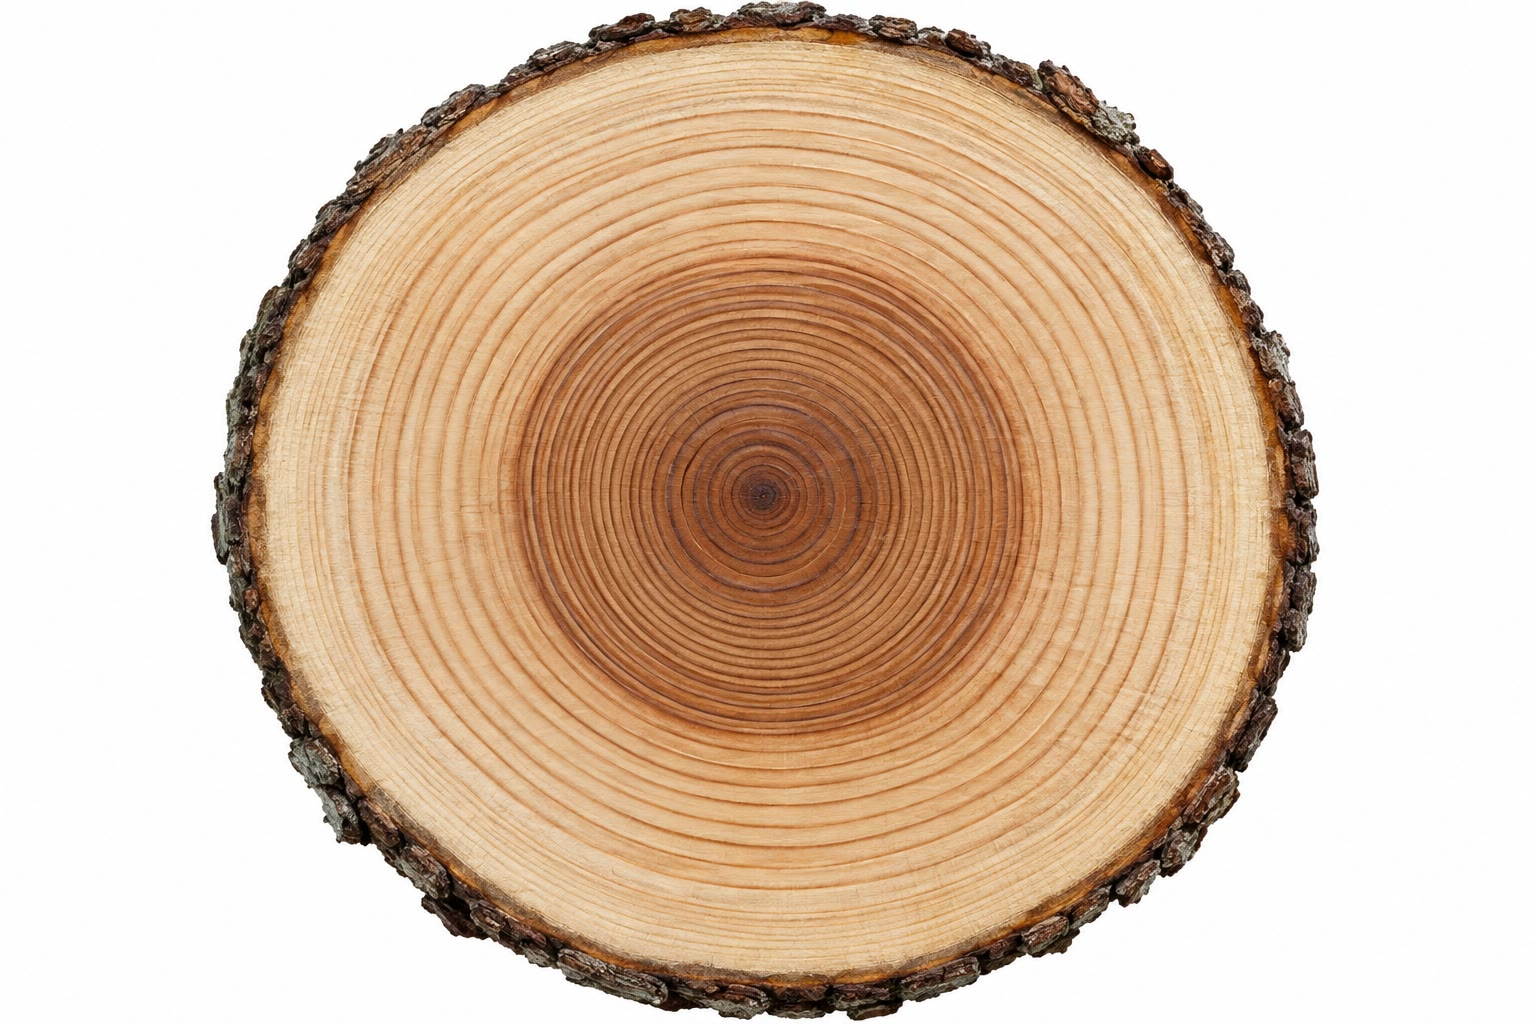
\includegraphics[width=0.5\linewidth]{images/book4/ai/b4-13-wood-rings.jpg}

{\small अनुप्रस्थ काट में चीड़ का एक तना: \omterm{def:b2:plant-meristems:wood}{वार्षिक वलय}, और हर एक
पूर्वकाष्ठ की एक फीकी तथा पश्चकाष्ठ की एक गहरी पट्टी, गहरा अंतःकाष्ठ,
और \omterm{def:b2:plant-meristems:wood}{छाल}।}
\end{omfigure}

\section{अभ्यास}

\begin{exercise}[$\star$]\label{exo:b2:plant-meristems:1}
\omterm{def:b2:plant-meristems:meristem}{विभज्योतक} की परिभाषा दीजिए, और किसी काष्ठीय पौधे के चारों \omterm{def:b2:plant-meristems:meristem}{विभज्योतक}
बताइए तथा हर एक क्या बनाता है।
\end{exercise}

\begin{exercise}[$\star$]\label{exo:b2:plant-meristems:2}
किसी मूल-शीर्ष के क्षेत्र टोप से ऊपर की ओर बताइए, और हर एक में किसी
कोशिका का क्या होता है। पार्श्व जड़ें कहाँ से आती हैं?
\end{exercise}

\begin{exercise}[$\star$]\label{exo:b2:plant-meristems:3}
थिमैन--स्कूग प्रयोग, उसका नियंत्रण और उसका निष्कर्ष
बताइए।
\end{exercise}

\begin{exercise}[$\star$]\label{exo:b2:plant-meristems:4}
किसी तने की काट में 60 वलय दिखते हैं, जिनमें बाहरी 15 फीके और बाक़ी गहरे
हैं। उस वृक्ष की आयु, उसके \omterm{def:b2:plant-meristems:wood}{रस-काष्ठ} की आयु, और यह बताइए कि तने का
कौन-सा भाग जीवित है।
\end{exercise}

\begin{exercise}[$\star\star$]\label{exo:b2:plant-meristems:5}
$\phi = \qty{0.1}{h^{-1}.MPa^{-1}}$, $Y = \qty{0.3}{MPa}$ के साथ,
$P = 0.4$, $0.6$ और \qty{0.8}{MPa} पर सापेक्ष वृद्धि दर और
हर एक पर दुगुना होने का काल निकालिए। कोई सूखा $P$ को \qty{0.25}{MPa} तक
गिरा देता है: क्या होता है?
\end{exercise}

\begin{exercise}[$\star\star$]\label{exo:b2:plant-meristems:6}
क्रमिक पत्तियाँ एक-दूसरे से \qty{137.5}{\degree} पर उठती हैं।
पत्तियों 1 से 8 की कोणीय स्थितियाँ (\qty{360}{\degree} के मापांक में)
निकालिए और दिखाइए कि पहली आठ में से कोई भी दो एक-दूसरे के
\qty{20}{\degree} के भीतर नहीं पड़तीं। यह उस पौधे के लिए क्यों मायने
रखता है?
\end{exercise}

\begin{exercise}[$\star\star$]\label{exo:b2:plant-meristems:7}
\qty{12}{m} ऊँचा कोई वृक्ष \qty{3}{mm} के वलय जोड़ता है। उस वर्ष जोड़ी
गई \omterm{def:b2:plant-meristems:wood}{काष्ठ} निकालिए जिसमें उसकी त्रिज्या \qty{5}{cm} है और उस वर्ष भी
जिसमें वह \qty{40}{cm} है, तथा उसके संगत कार्बन (शुष्क घनत्व
\qty{500}{kg/m^3}, आधा कार्बन)।
\end{exercise}

\begin{exercise}[$\star\star$]\label{exo:b2:plant-meristems:8}
किसी \emph{clv3} उत्परिवर्ती, किसी \emph{wus} उत्परिवर्ती, और दोहरे
उत्परिवर्ती के \omterm{def:b2:meiosis-heredity:vocabulary}{लक्षण-प्ररूपों} की भविष्यवाणी कीजिए, और दोहरे उत्परिवर्ती
से उस चक्र में दोनों जीनों का क्रम समझाइए।
\end{exercise}

\begin{exercise}[$\star\star$]\label{exo:b2:plant-meristems:9}
ऑक्सिन \qty{1}{cm/h} पर ढोई जाती है; ऊतक में उसका विसरण गुणांक
\qty{1e-9}{m^2/s} है। शीर्ष से \qty{20}{cm} नीचे की किसी कलिका तक वह
संकेत अभिगमन से और विसरण से कितने समय में पहुँचता है
($t = x^2/2D$)? ध्रुवीय अभिगमन उस पौधे को क्या देता है?
\end{exercise}

\begin{exercise}[$\star\star\star$]\label{exo:b2:plant-meristems:10}
मक्का की कोई जड़ प्रतिदिन \qty{3}{cm} बढ़ती है। \omterm{def:b2:plant-meristems:meristem}{विभज्योतक} कोशिकाएँ
\qty{20}{\micro m} लंबी हैं और परिपक्व होने से पहले दस गुना लंबी हो जाती
हैं; और हर कोशिका-पंक्ति में लगभग \num{100} विभाजित होती कोशिकाएँ हैं।
हर पंक्ति के \omterm{def:b2:plant-meristems:meristem}{विभज्योतक} को प्रतिदिन कितनी कोशिकाएँ बनानी पड़ती हैं, और
उससे कौन-सा कोशिका-चक्र काल निकलता है?
\end{exercise}

\begin{exercise}[$\star\star\star$]\label{exo:b2:plant-meristems:11}
1960 के दशक के अर्ध-बौने गेहूँ ऐसे \omterm{def:b2:genome-diversification:mutation}{उत्परिवर्तन} ढोते हैं जो उस
पौधे को जिबरेलिन के प्रति असंवेदी बना देते हैं। समझाइए कि वे छोटे क्यों
हैं, कोई छोटा पौधा भारी खाद पर अधिक दाना क्यों दे सकता है, और
किसी जंगली पौधे में वही \omterm{def:b2:genome-diversification:mutation}{उत्परिवर्तन} हानि क्यों होता।
\end{exercise}

\begin{exercise}[$\star\star\star$]\label{exo:b2:plant-meristems:12}
``कोई प्राणी एक बार गढ़ा जाता है; कोई पौधा जीवन भर गढ़ा जाता है।''
विभज्योतकी वृद्धि के उन परिणामों पर विचार कीजिए जो किसी पौधे की अपने
पर्यावरण के उत्तर देने, क्षति झेलने और सहस्राब्दियों जीने की क्षमता के
लिए हैं --- और उस रणनीति का एक दाम भी।
\end{exercise}

\section{समस्या: संख्याओं में एक वृक्ष}

\begin{problem}[{सप्तांत समस्या --- किसी युवा वृक्ष का वर्ष भर पीछा:
उसके शीर्ष कितनी पत्तियाँ बनाते हैं, लॉकहार्ट के नियम से किसी
पर्वसंधि-अंतराल की वृद्धि, उसका विभज्योतक कितनी काष्ठ बिछाता है और उसका
कार्बन-मूल्य, और छँटाई पर उसकी कलिकाओं की अनुक्रिया, और अंत प्रति वर्ष
पत्तियों, पर्वसंधि-अंतराल की प्रति घंटा वृद्धि और वर्ष की काष्ठ पर}]
\label{pb:b2:plant-meristems:1}
किसी युवा लिंडेन वृक्ष के \num{200} बढ़ते प्ररोह-शीर्ष हैं; और हर शीर्ष
\num{150}-दिन की ऋतु में हर \num{3} दिन पर, \qty{137.5}{\degree} के
अंतराल पर, एक पत्ती आरंभ करता है। कोई बढ़ता पर्वसंधि-अंतराल \qty{2}{cm}
लंबा है, और उसकी कोशिकाओं का $\phi = \qty{0.05}{h^{-1}.MPa^{-1}}$, $Y =
\qty{0.35}{MPa}$ है; स्फीति दिन में \qty{0.55}{MPa} और
रात में \qty{0.75}{MPa} रहती है (\qty{12}{h} प्रत्येक)। वह तना
\qty{8}{m} ऊँचा और \qty{10}{cm} त्रिज्या का है; \omterm{def:b2:plant-meristems:meristem}{विभज्योतक} प्रति वर्ष
\qty{5}{mm} जोड़ता है; और शुष्क \omterm{def:b2:plant-meristems:wood}{काष्ठ} \qty{500}{kg/m^3} तथा आधा कार्बन है।
उस मुकुट में \qty{80}{m^2} पत्तियाँ हैं जो \num{150} दिनों तक प्रति वर्ग
मीटर प्रतिदिन शुद्ध \qty{4}{g} कार्बन स्थिर करती हैं।

\medskip
\noindent\textbf{भाग I --- पत्तियाँ।}
\begin{enumerate}
  \item एक शीर्ष एक ऋतु में कितनी पत्तियाँ बनाता है? और पूरा
        वृक्ष?
  \item किसी एक प्ररोह पर पत्तियों 1 से 5 की कोणीय स्थितियाँ निकालिए।
  \item कितनी पत्तियों के बाद कोई पत्ती पत्ती 1 के
        \qty{10}{\degree} के भीतर पड़ती है? (\qty{137.5}{\degree} के
        गुणज आज़माइए।)
  \item वह स्वर्णिम कोण उस पौधे के लिए क्या साधता है, और किस हॉर्मोन
        का अभिगमन उसे बनाता है?
  \item यदि हर पत्ती का क्षेत्रफल \qty{80}{cm^2} हो, तो वह वृक्ष एक
        ऋतु में कितना पर्ण-क्षेत्रफल गढ़ता है? मध्य-ग्रीष्म में वह जो
        \qty{80}{m^2} ढोता है उससे तुलना कीजिए।
  \item वह वृक्ष पर्णपाती है। वह हर वसंत अपने पर्ण-क्षेत्रफल का कितना
        अंश फिर गढ़ता है, और पहली पत्तियों का कार्बन कहाँ से आता है?
  \item कोई \emph{clv3} \omterm{def:b2:genome-diversification:mutation}{उत्परिवर्तन} हर शीर्ष का आकार तिगुना कर देता है।
        प्रश्न 1 और 5 के उत्तरों में क्या बदलता, और वे प्ररोह कैसे
        दिखते?
\end{enumerate}

\medskip
\noindent\textbf{भाग II --- एक पर्वसंधि-अंतराल।}
\begin{enumerate}[resume]
  \item दिन की और रात की सापेक्ष वृद्धि दर निकालिए।
  \item \qty{2}{cm} से आरंभ करके एक दिन में और एक रात में जुड़ी लंबाई
        निकालिए।
  \item ऐसे चार दिनों में उस पर्वसंधि-अंतराल की लंबाई क्या है?
        (वृद्धि को चक्रवृद्धि मानिए, $L(t) = L_0 e^{rt}$, माध्य दर के साथ।)
  \item कोई जिबरेलिन उपचार $Y$ को गिराकर \qty{0.25}{MPa} कर देता है।
        दिन तथा रात की दरें फिर से निकालिए।
  \item कोई सूखा स्फीति को दिन-रात \qty{0.4}{MPa} पर रोक देता है।
        वह दर निकालिए, और बताइए कि परासरणी समायोजन क्या करता है।
  \item समझाइए कि प्रकाशसंश्लेषण दिन में होने पर भी रात की वृद्धि दिन की
        वृद्धि से अधिक क्यों है।
\end{enumerate}

\medskip
\noindent\textbf{भाग III --- \omterm{def:b2:plant-meristems:wood}{काष्ठ}।}
\begin{enumerate}[resume]
  \item इस वर्ष जुड़ी \omterm{def:b2:plant-meristems:wood}{काष्ठ} का आयतन और उसका शुष्क द्रव्यमान निकालिए।
  \item उसमें कार्बन निकालिए।
  \item उस ऋतु में मुकुट द्वारा स्थिर किया गया कार्बन निकालिए।
  \item मुकुट के कार्बन का कितना अंश तने की \omterm{def:b2:plant-meristems:wood}{काष्ठ} में गया?
        तीन और सिंक बताइए।
  \item बीस वर्ष में, उसी वलय-चौड़ाई पर, वार्षिक
        काष्ठ-वृद्धि क्या होगी? वह चढ़ती क्यों है?
  \item उस तने के दो वलय अपने पड़ोसियों से आधी चौड़ाई के हैं। दो कारण
        सुझाइए और यह भी कि कोई वृक्षकालक्रमविज्ञानी उन्हें कैसे अलग
        पहचानेगा।
\end{enumerate}

\medskip
\noindent\textbf{भाग IV --- कलिकाएँ और छँटाई।}
\begin{enumerate}[resume]
  \item वह माली हर प्ररोह-शीर्ष काट देता है। कक्षस्थ कलिकाओं की
        अनुक्रिया और महीने भर में उस वृक्ष के आकार की भविष्यवाणी कीजिए।
  \item हर कटान पर ऑक्सिन का लेप उस अनुक्रिया को कैसे बदलेगा?
  \item कोई बाड़ वर्ष में छह बार काटी जाती है। \omterm{prop:b2:plant-meristems:apical}{शीर्ष प्रभाविता} से
        समझाइए कि वह घनी क्यों हो जाती है।
  \item ठूँठ तक काटा गया कोई वृक्ष एक दर्जन प्ररोह फिर उगा लेता है। वे
        कहाँ से आते हैं, और कोई पौधा अपने हर प्ररोह की हानि क्यों झेल
        सकता है जबकि कोई प्राणी अपने सिर की हानि नहीं झेल सकता?
  \item जड़ों को पानी मिलने के बाद उनसे साइटोकाइनिन चढ़ती है।
        कलिका के निकलने पर उसके प्रभाव की भविष्यवाणी कीजिए।
  \item परिणाम बताइए: प्रति शीर्ष और प्रति वृक्ष प्रति ऋतु पत्तियाँ,
        पर्वसंधि-अंतराल की दिन तथा रात की वृद्धि दरें, और वर्ष की
        \omterm{def:b2:plant-meristems:wood}{काष्ठ} तथा कार्बन।
\end{enumerate}
\end{problem}
